Blablabla distribuciones comunes para variables discretas:

\begin{figure}[H]
    \begin{subfigure}{.5\textwidth}
        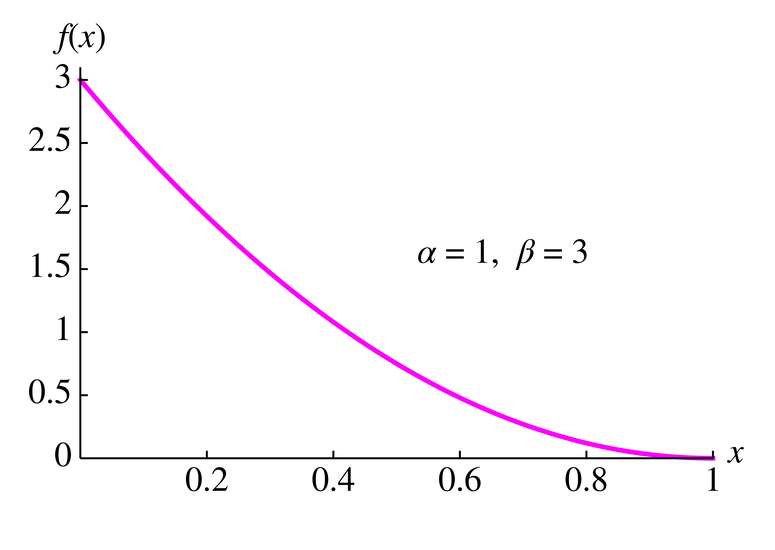
\includegraphics[width=1\linewidth]{beta.png}
        \caption{Beta}
    \end{subfigure}
    \begin{subfigure}{.5\textwidth}
        \includegraphics[width=1\linewidth,right]{binominal.png}
        \caption{Binominal}
    \end{subfigure}
\begin{subfigure}{.5\textwidth}
\includegraphics[width=1\linewidth]{negativabinominal.png}
\caption{Negativa binominal}
\end{subfigure}
    \begin{subfigure}{.5\textwidth}
        \includegraphics[width=1\linewidth]{epsilon_lambda.png}
        \caption{$\epsilon(\lambda)$}
    \end{subfigure}
    \begin{subfigure}{.5\textwidth}
        \includegraphics[width=1\linewidth]{gama.png}
        \caption{$\Gamma$}
    \end{subfigure}
    \begin{subfigure}{.5\textwidth}
        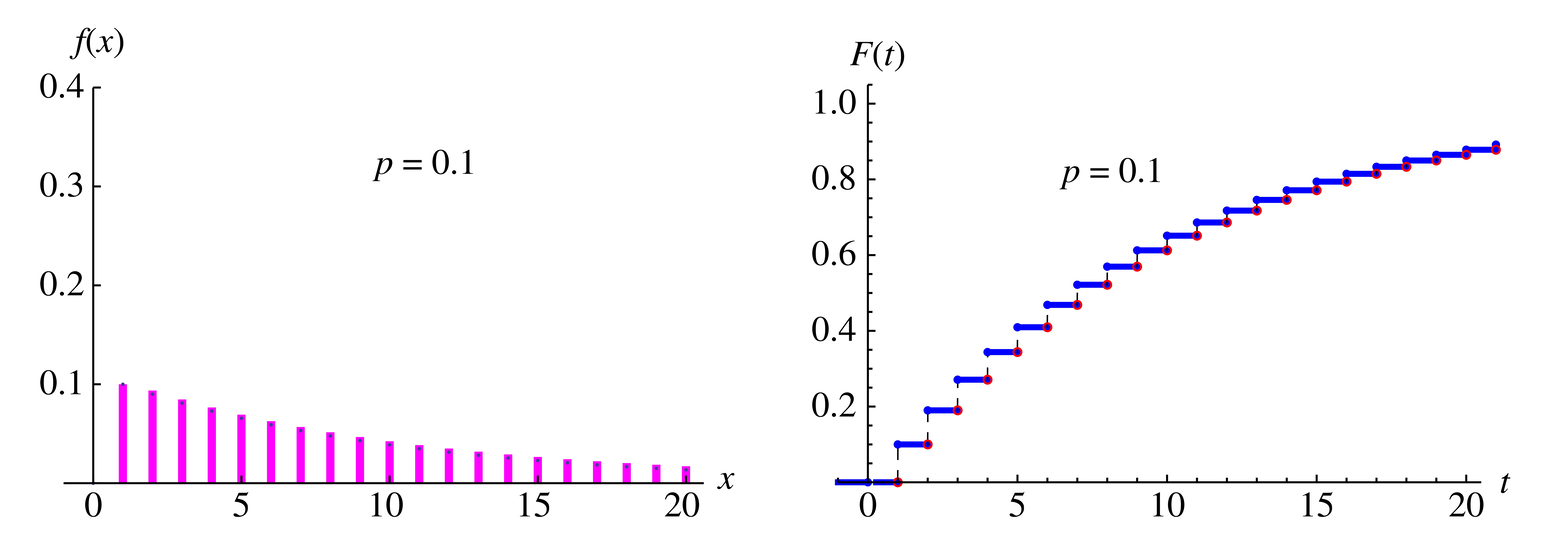
\includegraphics[width=1\linewidth]{geom.png}
        \caption{Geométrica}
    \end{subfigure}
    \begin{subfigure}{.5\textwidth}
        \includegraphics[width=1\linewidth]{hyperg.png}
        \caption{Hipergeométrica}
    \end{subfigure}
    \begin{subfigure}{.5\textwidth}
        \includegraphics[width=1\linewidth]{normal.png}
        \caption{Normal}
    \end{subfigure}
    \begin{subfigure}{.5\textwidth}
        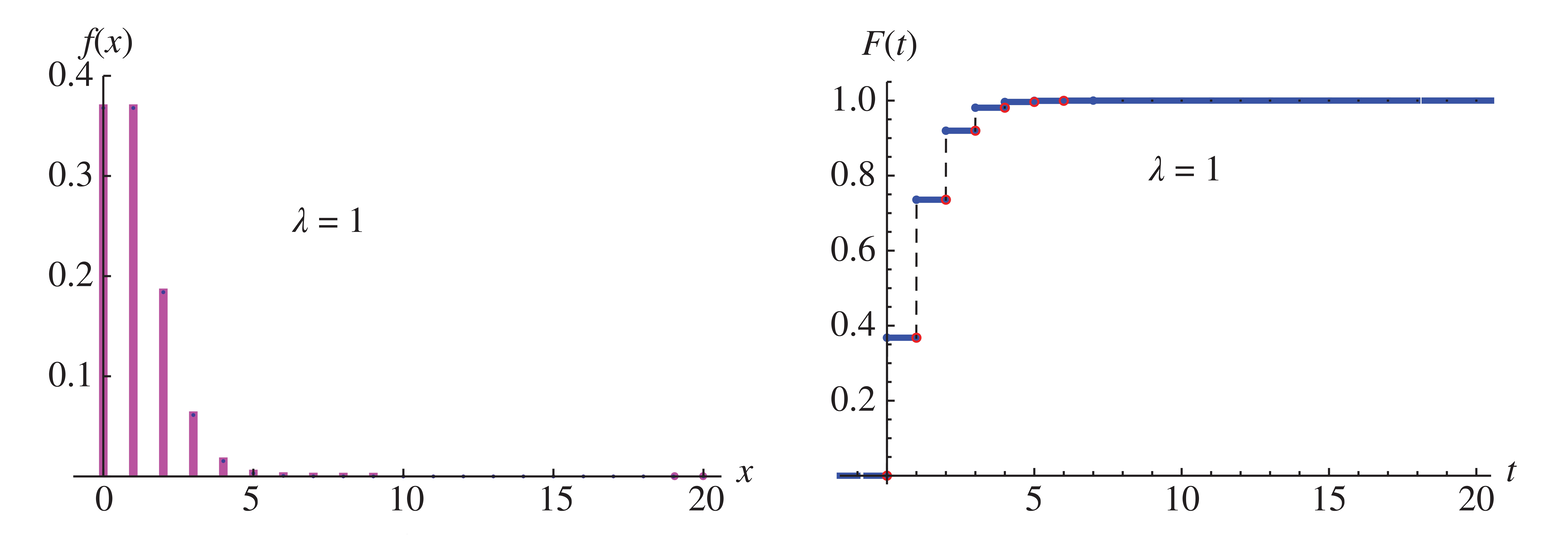
\includegraphics[width=1\linewidth]{poisson.png}
        \caption{Poisson}
    \end{subfigure}
    \begin{subfigure}{.5\textwidth}
        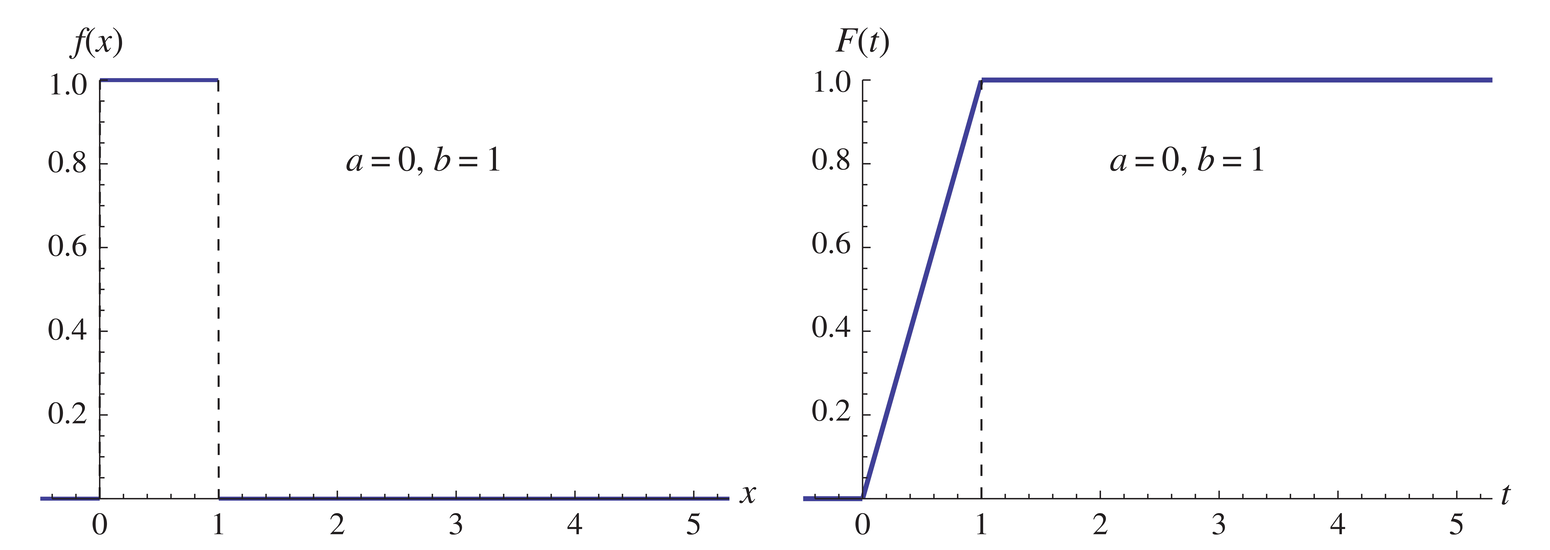
\includegraphics[width=1\linewidth]{uniforme.png}
        \caption{Uniforme}
    \end{subfigure}
\end{figure}